\chapter{Encoding FEC Chain} \label{chap:encoder}

% In this document explain all the things which I have done until the midterm presentation.
% All the details, Optimization techniques I have employed.
% Following text might be useful for writing the text.
% Also my midterm presentations/office presentations will be really useful for writing this part.  
% Reference paper for explaining the different components of the this FEC chain "Design of Polar codes for 5G NR radio"

%Work I have done Until now.
%
%%****************Optimizations to the original implementations until now.
%%****************Generic optimizations
%- Using optimization primitives such as likely and unlikely.
%- Aligning memory to 32 bytes so copying of data can be vectorized.
%- Polar transform optimization	
%- Replace binary additions with xor. instead of addition and then modulus two.
%- division and multiplications by left and right shift operations.
%- Avoided copy operations in polarTransform operations.
%****************Optimization in getting reliability indices.
%- Avoided remove and erase operations which have huge overhead. Wrote a efficient mechanism(reduced the latency by 176 us).
%- Instead removing and erasing I mark the element as removed.
%- Since the reliability indexes won't change. I built a look up table in place of searching all (1024)indices reduced the latency by 40us
%- Avoided copying operations of interleaved indexes.
%- Unrolled the loop to reduce the jumps.
%****************Rate matching optimizations.
%- optimization in subblock interleaving, Rewrote the logic to avoid E number of division and modulus operations.
%- Unrolled the for loops in subblock inteleaving method.
%- Implemented optimal version of bit selection, Avoided E number of modulus operations which are very costly.
%- Again optimization primitives for helping the branch predictor.
%
%
%Fast version of Encoding API's.
%In the original implementation of the polar encoding each of the bit is treated as 32 bit integer. This is highly inefficient
%when the goal is to process multiple bits at time. With each bit considered as 32 bit integer SIMD instructions won't provide
%any performance improvement. Reason is SIMD instruction can process multiple bits at time. avx2 instructions 256bits at a time.
%if we have 32 bits to represent a single bit. we can process only 8 bits at time. Which doesn't significantly improve the
%performance. To avoid this disadvantage and make use of SIMD capability. each 64 bit integer is considered as 64 bits of data.
%so one avx2 instruction can process 256 data bits in a single instruction.
%- Built a look up table to avoid last eight stages of polar encoding instead of traversing till end of tree.
%- Implemented SIMD instruction based encoding. Encoding happens within 0.6 us for N = 512.
%- Implemented optimal version of CRC calculation which can calculate CRC for PDCCH chain within 0.8 us. Original implementation was taking 7 us.
%- Implemented a bit interleaver which can deal with this format of data.

In the 5G standard, polar codes are used in the downlink to encode downlink control information (DCI) over physical downlink control channel (PDCCH) and for Master Information Block (MIB) in the physical broadcast channel (PBCH). In the uplink, to encode uplink control information (UCI) over the physical uplink control channel (PUCCH) and physical uplink shared channel (PUSCH). In this work, notations introduced in 3GPP technical specification \cite{3gpp.38.212} are used.

This chapter presents the details of the polar encoding FEC chain in 5G with a block diagram. Future sections will explain the functionality and potential latency contribution of individual components in the FEC chain. Each of these individual components is extensively profiled to identify expensive operations and latency contribution. After identifying the bottlenecks, both algorithmic and software optimization techniques are employed. Algorithm optimizations include reformulation of the problem to avoid expensive operations, encoder tree pruning using lookup tables etc. Huge latency reduction is achieved through software optimizations as well. Some of the major software optimization methods are unrolling an encoder function, exploiting data parallelism with SIMD, avoiding exponentially complex operations and finally reformulation of polar code construction to avoid expensive remove, erase and copying operations.

% code profiling/latency measurement methods, software/algorithm optimizations employed to the FEC chain, SIMD feature of the modern processors is exploited to obtain the low latency for PBCH and PDCCH FEC chains and frozen set selection algorithm improvement with the aid of look up table, finally presents the encoding process as traversal of a binary tree and how the encoding latency can be improved by pruning the tree hence avoiding the tree traversal instead using a lookup table to obtain the encoded result.

Figure ~\ref{fig:5g_txfec_chain} represents the complete polar FEC chain for PBCH and PDCCH. In general, $A$ bits have to be transmitted with a code of length $E$ bits. $L$ CRC bits are added to the information bits, resulting in  $K = (A + L)$ bits. The Resulting $K$ bits are then passed through an input bit-interleaver. Interleaved bits are concatenated with parity bits. In the next step information bit indices are identified and the information bits are inserted in those positions to obtain a vector $\boldsymbol{u}$ of length $N$, where $N = 2^{n}$. Encoding is performed with a mother code with parameters $(N, K)$. Encoding is performed through $\boldsymbol{d = uG_{N}}$, where the generator matrix $\boldsymbol{G_{N} = G^{\otimes n}}$ obtained by $n^{th}$ Kronecker product of Ar\i kan matrix. The codeword $\boldsymbol{d}$ is passed through a subblock interleaver. It divides the codeword into 32 blocks and performs interleaving. The interleaving pattern is given in Figure \ref{fig:subblockInterleaver}. The next step involves rate matching, which maps mother code block-length $N$ to rate matching size $E$ bits. Rate matching can be repetition, puncturing or shortening.  This decision is taken based on the value of $E$, $N$, and $K$. when $E > N$ repetition is applied. For repetition, some parts of the code word are repeated to create $E$ bits from $N$ bits. For the case $E < N$ either shortening or puncturing is applied. In this mode, bits are discarded to create $E$ bits from $N$. Finally, channel interleaving is performed to improve the error correction performance for higher order modulations. This chapter dives into the implementation details of each block in an algorithmic level with small code snippets whenever necessary. It also analyzes the bottlenecks and presents solutions through different optimization techniques. All the latency measurements in this section are performed on AMD EPYC processor running at 1.6 GHz with Turbo disabled. Turbo mode allows the processor to dynamically increase the frequency when the load is high, To get accurate measurements, Turbo mode is disabled.

%Analyzes latency introduced by different blocks of FEC chain and also presents the algorithmic and platform specific optimizations.

\begin{figure}[h]
	\centering
	\includegraphics[width=0.7\textwidth]{./figures/5GFECChain.pdf}
	\caption{Polar Encoding FEC chain for PDCCH/PBCH}
	\label{fig:5g_txfec_chain}
\end{figure}

\begin{figure}[h]
	\centering
	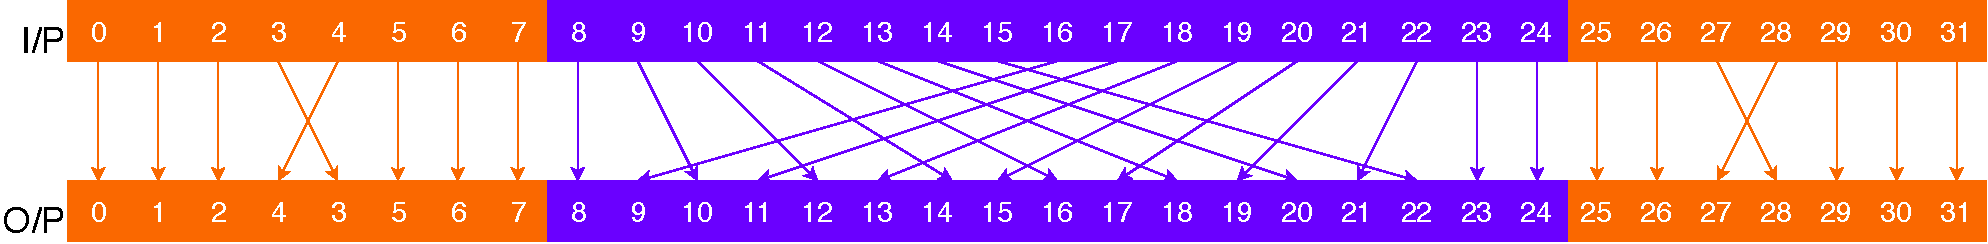
\includegraphics[width=1\textwidth]{./figures/subblockInterleaver.pdf}
	\caption{Subblock Interleaver for PDCCH/PBCH}
	\label{fig:subblockInterleaver}
\end{figure}

\section{Data packing and Unpacking operations} \label{dataPackUnpack}
Typically in software implementations, for clarity and ease implementation each bit of information is represented with 32-bit or 64-bit integers. Due to the presence of only one bit of information in each integer, if 1024 bits need to be encoded or decoded then 1024 integers are involved in encoding or decoding process. However, this isn't the case in hardware implementations since each bit can be processed in hardware description languages (HDL). Representing one bit of information using a 32 or 64-bit integer has the following disadvantages.

\begin{description}[font=$\bullet$~\normalfont]
	\item Increased memory footprint: For 1024 bits, $64\cdot1024$ bits memory need to be allocated. It is equivalent to 8 kilobytes. Allocating and initializing this memory can introduce significant latency.
	\item Results in more cache misses: If more memory is allocated, more data needs to accessed from RAM which can result in more cache misses.
	\item Serializes encoding/decoding: General purpose processors have a data path width of 64-bit. If each bit is represented using a 64-bit integer, we are not using the capability of processing 64 bits simultaneously. Instead, each bit is processed sequentially. This can make encoding or decoding sequential although the processor is capable of processing multiple bits in parallel.
\end{description}

To avoid the above disadvantages and to enable data parallelism, this work tries to pack multiple bits into a single integer. Although packing multiple bits to a single integer has advantages, for some operations such as bitwise interleaving accessing each bit efficiently is very important. To exploit the advantages of bit packing as well as the advantages of accessing each bit separately, it is necessary to convert between the two. This is where the power of SIMD instructions in modern processors comes into play. These processors come with special hardware instructions which help to efficiently pack and unpack data. Data bits are used in packed format when data parallelism needs to be exploited and in unpacked format when certain operations require bits to be accessed individually. These pack/unpack instructions are very efficient and have low latency. Details of the AMD EPYC processor's instructions with corresponding latencies are provided in \cite{AgnerFog}.

Some instructions which are used for fast packing and unpacking are:
\begin{code}
	\captionof{listing}{Sample packing/unpacking instructions}
	\label{code:samplepackUnpack}
\begin{minted}[frame=single]{c++}
	int _mm_movemask_pi8(__m64 a);
	int _mm_movemask_epi8(__m128i a);
	__m256i _mm256_unpackhi_epi8(__m256i a, __m256i b);
	/** many more **/
	
\end{minted}
\end{code}


\begin{code}
	\captionof{listing}{Sample packing/unpacking example}
	\label{code:packUnpackExample}
	\begin{minted}[frame=single]{c++}
template<>
inline int8_t packBits<8>(int8_t s[]) {
	__m64 v8 = _mm_set_pi8(s[0],s[1],s[2],s[3],s[4],s[5],s[6],s[7]);	
	uint8_t idx = _mm_movemask_pi8(_mm_slli_si64(v8, 7));
}
\end{minted}
\end{code}

Listing \ref{code:packUnpackExample} shows an example of bit packing. It receives vector of size 8, containing 8-bit integers each representing a bit. Returns a one bit-packed one 8-bit integer.

\section{CRC calculation}
%Explain why CRC attachment is considered in whole FEC chain, how it is useful for decoding polar codes. Explain algorithmic complexity of CRC calculation, How much time it was taking, How the optimization is carried out to reduce the CRC calculation time.
In the polar FEC chain as shown in the Figure \ref{fig:5g_txfec_chain}, an L-bit CRC is calculated for $A$ information bits and attached to the message. The number of CRC bits (L) varies for different physical channels. In the downlink, for the payload of PBCH/PDCCH, 24-bit CRC is used. The Uplink Control Information (UCI) uses a 6-bit or 11-bit CRC based on the value of $A$. For $12 \leq A \leq 19$ and $A \geq 20$ 6-bit CRC and 11-bit CRC are used respectively. The polynomials for different CRC values are shown below \cite{3gpp.38.212}.

\begin{equation} \label{crc_polynomial6}
g_{6}(x) = x^{6} + x^{4} + 1
\end{equation}
\begin{equation} \label{crc_polynomial11}
g_{11}(x) = x^{11} + x^{10} + x^{9} + x^{5} + 1
\end{equation}
\begin{equation} \label{crc_polynomial24}
g_{24}(x) = x^{24} + x^{23} + x^{21} + x^{20} + x^{17} + x^{13} + x^{12} + x^{8} + x^{4} + x^{2} + x + 1
\end{equation}

Information bits concatenated with CRC increases the error correction performance of polar codes significantly. CRC is used for selecting the correct codeword out of potential candidates in the list. With CRC aided decoding, polar codes performance better than LDPC and Turbo codes at short block-lengths. To reduce the latency of encoding FEC chain CRC needs to be calculated very efficiently. A naive implementation of CRC calculation uses a shift register. This method calculates the CRC sequentially for one bit at a time as given in \cite{naiveCRCCalculation}. As explained in Section \ref{dataPackUnpack}, it is very inefficient to process bits sequentially. Algorithm in \cite{Sarwate:1988:CCR:63030.63037} is adapted to calculate the CRC for the polynomial in \eqref{crc_polynomial24} using lookup table based approach. This algorithm calculates the CRC blockwise with the help of the lookup table. In other words, divide the data into blocks of $B$-bits, read the corresponding CRC value from a lookup table and combine the individual CRC's of the blocks in a predefined way to create a CRC for complete data. Data bits are divided into blocks of 8-bits and packed into 8-bit integers. The CRC value corresponding to 8-bit integer is read from the lookup table and combined with CRC of a previous 8-bit integer. This process continues until CRC is calculated for all data bits. If the number of data bits are not multiple of 8 then zero's are appended at the MSB position.  Table \ref{tab:crcLatencyTable} presents the latency values of naive and optimized  CRC calculation methods for payload of 41-bits. There is a significant improvement in the optimized method compared to naive implementation.

\begin{table}[h!]
	\begin{center}
		\caption{CRC24 calculation latency comparison}
		\label{tab:crcLatencyTable}
		\begin{tabular}{c|c|c} % <-- Alignments: 1st column left, 2nd middle and 3rd right, with vertical lines in between
			\textbf{ } & Naive & Optimized \\
			\hline
			Latency ($\mu$s) & $7.7$ & $0.016$\\
		\end{tabular}
	\end{center}
\end{table}

After CRC attachment total number of information bits become $K = A + L$, where $ A $ is data bits and $ L $ is CRC size.

\section{Input Bit Interleaver}
Information bit stream of length $A$ is attached with CRC ($L$) and is interleaved by the input bit interleaver to create a distributed-CRC. This step is necessary for the early termination of decoding at the receiver if CA-SCL (CRC aided SCL) is used. The interleaving pattern is designed in such a way that every CRC remainder bit is placed after its relevant information bits. This helps to discard some paths in the list decoding process if the CRC calculated from the previously decoded information bits doesn't match the CRC bit. In other words, the input bit interleaver distributes CRC to ease decoding when a list decoder used through early termination. The interleaving pattern is calculated at runtime since it depends on the number of information bits ($K$). In this part of the implementation, there is not much optimization performed in this work since interleaving needs to carried out sequentially and also due to the fact that $K$ is not very large. Complete details of the input bit interleaver and interleaving pattern calculation can be found in \cite{3gpp.38.212}.

\section{Polar Code Construction}
Polar code construction is the process of identifying information and frozen bit position, i.e $K$ out of $N$ positions. This step determines the error correction performance of polar codes. There are many methods in the literature to construct polar codes. Ar\i kan \cite{Arikan} proposed to use the Bhattacharyya parameter as reliability metric for Binary Erasure Channels (BEC) then deriving reliability values using Monte Carlo simulation. For other channels, Mori and Tanaka \cite{MoriTanakaDE} use more accurate density evolution (DE) methods but it suffers huge complexity. Tal and Vardy proposed Gaussian Approximation (GA) to reduce the complexity of DE with approximations \cite{TalVardyGA}. Still, the GA method has a high computational complexity which scales linearly with code block-length, therefore, it is unacceptable for varying SNR, block-length and code rate. In use cases such as 5G, where the channel is continuously varying. it is not feasible to construct polar codes on the fly due to stringent latency requirements of both encoder and decoder. The polar code construction in 5G takes a suboptimal approach, instead of constructing polar codes for every different SNR, block-length and code rate, construction is carried out in such a way that the constructed code performs sufficiently good over a large range of SNR, block-length and code rate. 5G polar code construction method is based on the contribution from Huawei which uses a $\beta$-expansion method with universal partial order (UPO) property of channel reliability as presented in \cite{betaExpansion}. \newline

The 5G standard has adopted five different polar code block-lengths. Block-length sizes $\mathcal{N}$ are by $\mathcal{N} = \{32,64,128,256,512,1024\}$.
For each of the block lengths, reliability indices values are specified in \cite{3gpp.38.212}. The polar code construction also depends on the rate matching mode since it affects the reliability of bit indices. The polar code construction is straightforward when rate matching output $E$ greater than or equal to block-length $N$. In such a case, code construction involves selection of $K$ most reliable indices for information bits remaining positions are frozen since bit reliability not affected by rate matching. Example  \ref{E_greaterThan_N} shows such a case. However when rate matching output size $E$ is smaller than block-length $N$ the selection of reliability indices becomes more involved which is described briefly in the next paragraph.

\subsubsection*{Polar code construction example for $N = 32, K = 16$ and $E = N$} \label{E_greaterThan_N}
Let's take an example with $N = 32$ channel reliability values are extracted from the reliability table provided in \cite{3gpp.38.212} and are given by

\begin{eqnarray*}
Q_{0}^{31} = \{ 0, 1, 2, 6, 3, 7, 9, 16,4, 8, 11, 17, 13, 19, 20, 26, 5, 10, 12, 18, 14, 21, 24, 27, 15, 23, 22, 28,\\
25, 29, 30, 31 \}
\end{eqnarray*}

The bit positions in reliability array $Q_{0}^{31}$ are ordered in increasing order of their reliability. For encoding with parameters $N = 32$ and $K = 16$, $K$ most reliable indices in the array i.e last 16 indices are used as information bit positions. 

\begin{eqnarray*}
	Q_{\textit{I}}^{\textit{K}} =  \{5, 10, 12, 18, 14, 21, 24, 27, 15, 23, 22, 28,25, 29, 30, 31 \}
\end{eqnarray*} 

For any other case, when $E < N$ either puncturing or shortening is performed during rate matching. Empirically it is been observed for polar codes that at low rates puncturing works better and shortening for high rates \cite{lowcomplexityPuncShorteng}. In 5G, it is not uncommon to have scenarios with rate matching output $E$ is less than block-length $N$. In such scenarios, some bits need to be discarded in the rate matching stage through puncturing or shortening. When encoded bits are discarded in the rate matching stage, the reliability of bit channels get affected, identifying reliable bits by taking effect of rate matching procedure makes polar code construction complex in terms of time. The naive implementation of reliability indices selection algorithm provided in \cite{3gpp.38.212} is carried out in C++ as shown in algorithm ~\ref{algo:polarCodeConstuctionAlgo}. Upon code profiling of encoder FEC chain implementation, it was found that polar code selection algorithm is the most time-consuming part among all the encoding FEC chain stages.

The following algorithm gives a simplified picture of functional implementation to select information bit indices by taking the effect of rate matching. 
Notations used in the algorithm are the same as the ones specified in 5G standard \cite{3gpp.38.212}.

$J(n)$ : Subblock interleaver pattern for a particular block-length $N$. \newline
$E$ \hspace{0.5cm}: Rate matcher output size. \newline
$N$ \hspace{0.45cm}: Mother code block length. \newline
$K$ \hspace{0.45cm}: Number of information bits.\newline
$Q_{\textit{0}}^{\textit{N-1}}$ : Reliability indices array for block-length $N$ in ascending order of reliability. \newline
$\overline{Q}_{\textit{I}}^{\textit{N}}$\hspace{0.25cm} : Information bit positions. \newline


\IncMargin{1.5em}
\begin{algorithm}[!h]
	\KwData{$Q_{\textit{0}}^{\textit{N-1}}$,$N$, $K$, $E$ and $J(n)$}
	\KwResult{$\overline{Q}_{\textit{I}}^{\textit{K}}$}
	$\overline{Q}_{\textit{F}}^{\textit{N}} = \emptyset$ \;
	\If {$\big(E < N\big)$} {
		\If {$\big((K\cdot 16) \leq (E\cdot 7)\big)$} {   %-------------------------------------------------> Puncturing
			$J_{sorted}(n) = sort(\{J(0),J(1),J(2)....J(N-E)\})$\;  \label{line:subblockRef1}
			\If {$\big(E \ge (0.75\cdot N)\big)$} {
				$size = \ceil*{\big[(3\cdot N\cdot 2 - E\cdot 4)/8\big]}$\;
				$\overline{Q}_{F}^{N} = J_{sorted}(n) \cup \{0,1,2, ... ,size-1\}$ \label{line:subblockRef2}
			} \Else {
				$size = \ceil*{\big[(9\cdot N\cdot 4 - E\cdot 16)/64\big]}$\;
				$\overline{Q}_{F}^{N} = J_{sorted}(n) \cup \{0,1,2, ... ,size-1\}$ \label{line:subblockRef3}
			}	
		} \Else {							    %-------------------------------------------------> Shortening
			$\overline{Q}_{F}^{N} = \{J_{sorted}(E), J_{sorted}(E + 1), ... J_{sorted}(N-1)\}$ \label{line:subblockRef4}
		}
	}
	$frozenSize = \big|\overline{Q}_{F}^{N}\big|$ \;
	$infoSize = N - frozenSize$ \;
	$Q_{\textit{I}}^{\textit{N}} = Q_{\textit{0}}^{\textit{N-1}}$ \;
	
	\For{$i=0$ to $frozenSize$} {
		$iterator = remove(Q_{\textit{I}}^{\textit{N}},\overline{Q}_{F,i})$ \;
		$erase(Q_{\textit{I}}^{\textit{N}},iterator)$ \;
	}
	$startIdxInfo = N - K - n_{PC}$ \;
	$\overline{Q}_{\textit{I}}^{\textit{K}} = \{Q_{\textit{I,startIdxInfo}},Q_{\textit{I,startIdxInfo + 1}},...,Q_{\textit{I,END}}\}$
	\caption{Polar code construction \cite{3gpp.38.212} Section 5.4}
	\label{algo:polarCodeConstuctionAlgo}
\end{algorithm}
\DecMargin{1.5em}

\IncMargin{1.5em}
\begin{algorithm}[!h]
	\KwData{$Q_{\textit{0}}^{\textit{N-1}}$,$N$, $K$, $E$ and $J(n)$}
	\KwResult{$\overline{Q}_{\textit{I}}^{\textit{K}}$}
	$\overline{Q}_{\textit{F}}^{\textit{N}} = \emptyset$ \;
	\If {$\big(E < N\big)$} {
		\If {$\big((K\cdot16) \leq (E\cdot7)\big)$} {   %-------------------------------------------------> Puncturing
			$J_{sorted}(n) = sort(\{J(0),J(1),J(2)....J(N-E)\})$\;  \label{line:OptisubblockRef1}
			\If {$\big(E \ge (0.75\cdot N)\big)$} {
				$size = \ceil*{\big[(3\cdot N\cdot 2 - E\cdot 4)/8\big]}$\;
			} \Else {
				$size = \ceil*{\big[(9\cdot N\cdot 4 - E\cdot 16)/64\big]}$\;
			}
			$\overline{Q}_{F}^{N} = J_{sorted}(n) \cup \{0,1,2, ... ,size-1\}$ \; \label{line:OptisubblockRef2}
			$frozenSize = length(\overline{Q}_{F}^{N})$ \;
			$mode = puncturing$ \;
		} \Else {							    %-------------------------------------------------> Shortening
			$frozenSize = N - E$ \label{line:OptisubblockRef4} \;
			$mode = shortening$ \;
		}
	}
	$Q_{\textit{I}}^{\textit{N}} = Q_{\textit{0}}^{\textit{N-1}}$ \;	
	\For{$i=0$ to $frozenSize$} {
		\If {$mode == puncturing$} {
			$index = lookUpTable[\overline{Q}_{F,i}]$\;
		} \Else {
			$index = lookUpTable[J[i + E]]$ \;
		}
		$Q_{I}^{N}[index] = $ INVALID \;
	}
	$idx = K$ \;
	\For{$i=size(Q_{I}^{N})$ to $0$} {
		$i = i-1$ \;
		\If {$Q_{I}^{N}[i]  \ne $INVALID} {
			$\overline{Q}_{\textit{I}}^{\textit{K}}[idx] = Q_{I}^{N}[i]$ \;
			$idx = idx-1$ \;
		}
	}
	\caption{Proposed optimized polar code construction}
	\label{algo:polarCodeConstuctionAlgoOptimized}
\end{algorithm}
\DecMargin{1.5em}

Algorithm \ref{algo:polarCodeConstuctionAlgo} shows how the information bit indices are selected by taking rate matching into account. Finding and removing incapable bits due to rate matching is an expensive operation. As it can be seen in the algorithm in lines ~\ref{line:subblockRef1}, ~\ref{line:subblockRef2}, ~\ref{line:subblockRef3} and ~\ref{line:subblockRef4} subblock interleaving pattern is also taken into account for identifying the incapable bits due to the presence of subblock interleaver between rate matching and encoder. Due to presence of time consuming operations such as $ sorting $, $ set\_union $, $ search $, $ remove $ and $ erase $. The contribution of this function highest among all the components of the FEC chain. In terms of latency, for a scenario with $E = 846, N = 1024, K = 130$ puncturing is required. For these parameters, the polar code construction, encoding, subblock interleaving rate matching and channel interleaver takes 411$\mu$s, only polar code construction contribution is 377 $\mu$s. \newline

Let's analyze the complexity of each the operations. Sorting is $\mathcal{O}\big((N-E)\log{}(N-E)\big)$ complex and of Set\_union is again $\mathcal{O}\big((N-E)\log{}(N-E)\big)$ complex \cite{cppStd}. The block-length $N$ is derived using $E$ and $K$, so $(N-E)$ is small compared to $N$. Next operation in the algorithm is $remove$ and $erase$. These functions are directly used from the standard C++ library. After deciding rate matching type (shortening/puncturing) and identifying incapable bit indices, these locations must be frozen, this requires traversing through reliability indices array and removing incapable bit locations. $remove$ and $erase$ functions are used to perform this operation. $remove$ function searches through a reliability array for incapable bit index and removes the element. $erase$ operation erases the memory allocated to removed element and resizes the array. The complexity of the remove operation is $\mathcal{O}(N)$. The $remove$ function has to search through all the elements of an array for every frozen value and have to move the elements to overwrite the removed position, the size of the array is $N$, it can be as large as $1024$. The erase operation has to deallocate the memory and resize the container. $remove$ and $erase$ together are $\mathcal{O}\big(N^2\big)$ complex. Above complexity-analysis is supported from latency measurements of $remove$ and $erase$ functions. It is found to be 318 $\mu$s. Avoiding these operations is critical to reducing the latency of the FEC chain. \newline

In this work, the algorithm is reformulated to avoid searching, copying and memory deallocation while removing incapable bit indices. To avoid search operations, a lookup table is built whose values indicate the position of particular reliability value. After identifying the position it is marked as removed instead of removing. Marking has two advantages first one is avoiding memory deallocation and copying, the second one is keeping the same order of elements which is particularly useful for using the same lookup table for finding the next incapable bit index. After all the incapable bit indices are marked as removed, only the unmarked elements are considered as reliable bit positions for placing information bits.

%Out of these positions information bits are placed in most reliable $K+n_{PC}$ positions.

The next optimization is avoiding copying subblock interleaving pattern to frozen indices array in case of shortening. Instead, a subblock interleaving pattern is directly used from the lookup table to mark the reliability indices as removed. In addition to above-mentioned optimizations, minor ones such as avoiding dynamic memory allocation instead reserving required memory in advance and employing pointer operations to avoid copying are performed. Finally, information bit positions are obtained from iterating the reliability table from the end (since indices are sorted in ascending order of reliabilities) and extracting $K$ unmarked positions. These optimizations reduced the latency of polar code construction from 377 $\mu$s to 15 $\mu$s.

Algorithm \ref{algo:polarCodeConstuctionAlgoOptimized} presents the optimized reformulation of algorithm \ref{algo:polarCodeConstuctionAlgo} without erase, remove, redundant copying operations and other minor optimizations.

Table \ref{tab:codeConstrLatency} comparison of latency for reliability indices selection function, for the FEC chain parameters $I_{IL} = 1, n_{max} = 10, n_{pc} = 0 ,n_{pc}^{wm} = 0, I_{BIL} = 0, E = 846, K = 130$. 
\begin{table}[!h]
	\begin{center}
		\caption{Latency comparison: Information bit positions selection}
		\label{tab:codeConstrLatency}
		\begin{tabular}{c|c|c} % <-- Alignments: 1st column left, 2nd middle and 3rd right, with vertical lines in between
			\textbf{ } & Naive & Optimized \\
			\hline
			Latency ($\mu$s) & $377$ & $15$\\
		\end{tabular}
	\end{center}
\end{table}

\section{Polar Encoding}
Once the information bit indices are identified, $K$ bits are inserted to reliable positions and remaining  $(N-K)$ are set to zero. Next step in the FEC chain is encoding. It can be carried out by multiplying $N$-bit vector with a generator matrix obtained by the $n^{th}$ Kronecker power of Arikan matrix $\utilde{G} = \big[\begin{smallmatrix} 1 & 0 \\ 1 & 1 \end{smallmatrix}$\big]  where $n$ is such that $N = 2^{n}$. State of the art direct row vector multiplication with matrix algorithm is $\mathcal{O}\big(N^{2.38}\big)$ complex \cite{MatrixMultComplexity}. However in case of polar codes generator matrix follows a regular structure, hence it is shown that encoding can be reduced to a recursive structure with a complexity of $\mathcal{O}(N\log{}N)$ \cite{Arikan}. There are different ways to visualize encoder, one is through the encoding circuit and another is through the tree structure. The latter is suitable when encoding is performed in hardware where a group of bits processed in parallel. Since this work focuses on implementation/optimization for software, the tree structure is considered. Example encoding visualized as a binary tree for $N = 8$ is illustrated in figure ~\ref{fig:treeEncoding}. Every node in a tree splits $i$-bit to $i/2$-bit vector and performs XOR of $0$ to $\frac{i}{2}-1$ bits with $\frac{i}{2}$ to $i-1$ bits. This process continues till bit vector length becomes one.

\begin{figure}[]
	\centering
	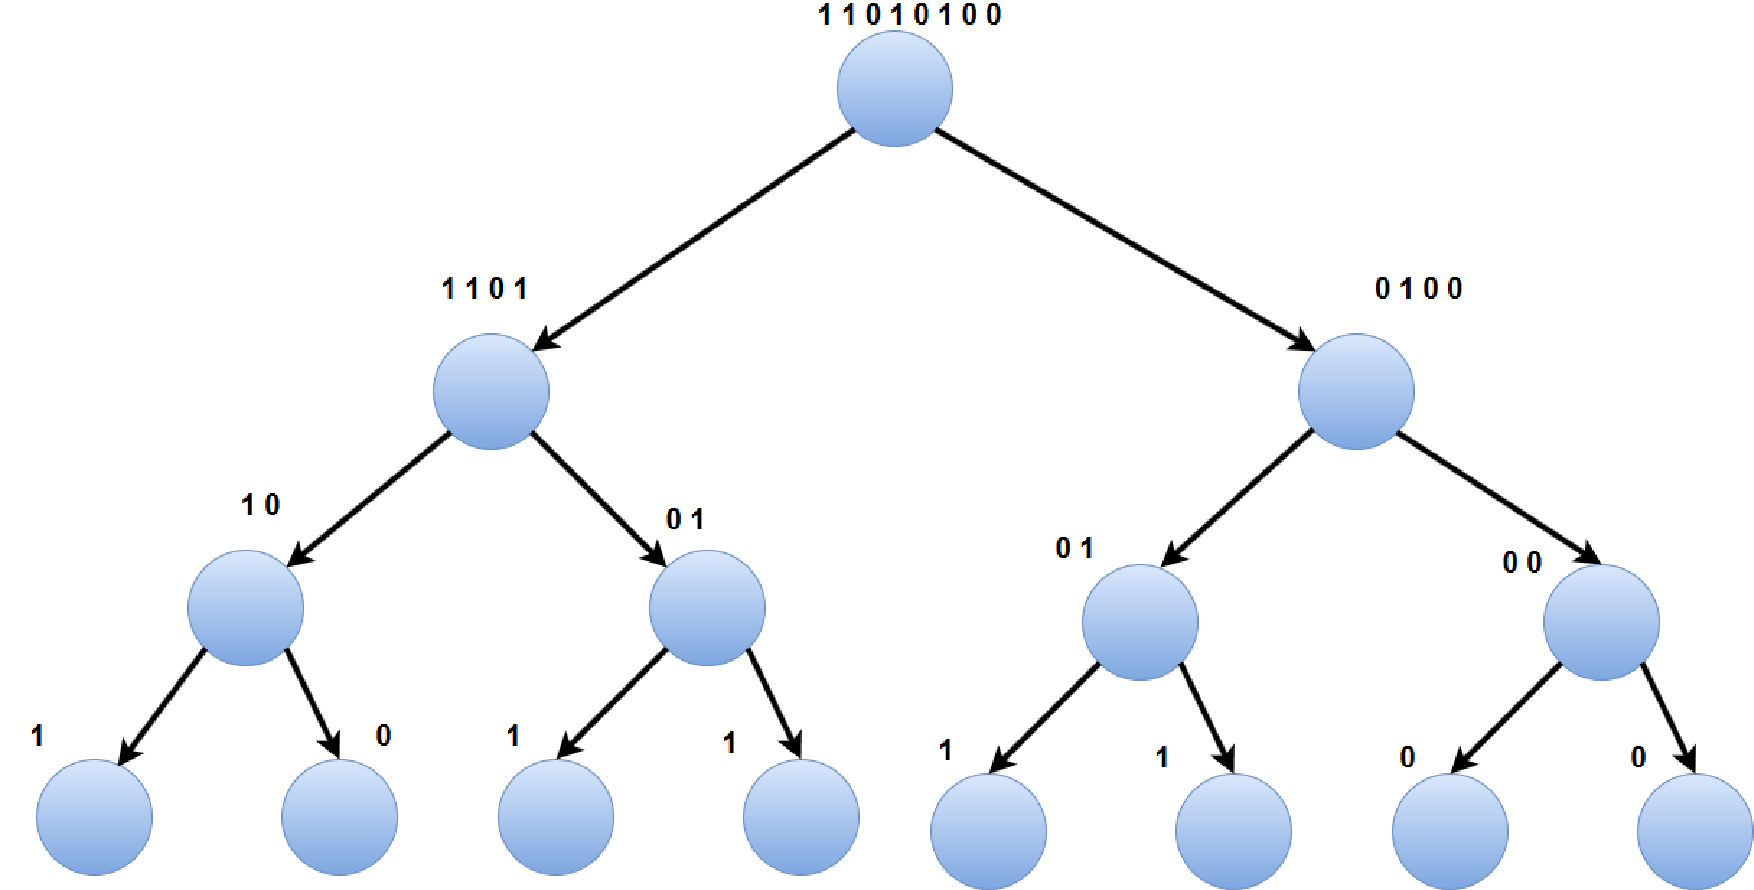
\includegraphics[width=0.7\textwidth]{./figures/treeEncoding.pdf}
	\caption{Encoding tree}
	\label{fig:treeEncoding}
\end{figure}

As it can be observed from the tree, the same operation is performed at every node only the size of a vector is different, due to the regular structure encoding problem fits the recursive algorithmic form. Algorithm ~\ref{algo:polarEncoder} shows a naive implementation of recursive encoder. In the algorithm, each bit is represented as one integer and each bit is processed serially, hence parallelism is not exploited. Upon profiling the implementation it also identified that ~\ref{line:copying1} and ~\ref{line:copying2} are also the bottlenecks since copying is involved. One more issue with the algorithm is recursive implementation. Although the encoding can be easily implemented in this way, each recursive function call in software is expensive, since it requires a new stack frame to be allocated. Background about the overhead of recursive function calling is presented in the previous chapter.

\IncMargin{1.5em}
\begin{algorithm}[!h]
	\KwData{$u_{\textit{0}}^{\textit{N-1}}$,$N$,$dIndex = 0$}
	\KwResult{$y_{\textit{0}}^{\textit{N-1}}$}
	\SetKwFunction{FMain}{recursiveEncode}
	\SetKwProg{Fn}{function}{:}{}
	\Fn{\FMain{$u_{\textit{0}}^{\textit{l-1}}$,$l$}}{
		\If {$l == 1$} {
			$y_{dIndex} = u_{0}$ \;
			$dIndex = dIndex + 1$ \;
		} \Else {
			$len = \frac{l}{2}$ \;
			$P_{\textit{0}}^{\textit{len-1}}$ = $u_{\textit{0}}^{\textit{len-1}}$ \; 	\label{line:copying1}
			$Q_{\textit{0}}^{\textit{len-1}} = u_{\textit{len}}^{\textit{l-1}}$ \;		\label{line:copying2}
			
			\For{$i=0$ to $length-1$} {													\label{line:xor1}
				$P_{\textit{i}} = P_{\textit{i}} \oplus Q_{\textit{i}}$\;				\label{line:xor2}
			}
			
			\FMain{$P_{\textit{0}}^{\textit{len-1}}$,$len$} \;
			\FMain{$Q_{\textit{0}}^{\textit{len-1}}$,$len$}	\;
		}
	}
	\caption{Naive polar encoder}
	\label{algo:polarEncoder}	
\end{algorithm}
\DecMargin{1.5em}

To avoid the disadvantages mentioned above, the following optimization techniques are considered.

$\bullet$ \textbf{Data parallelism} To avoid the serial processing of bits and hence to improve the parallelism factor, the method described in Section ~\ref{dataPackUnpack} is used, i.e, multiple bits are packed to a single integer. In this particular instance, every 64 bits are packed into 64-bit integers so that 64-bits can be processed in parallel with a 64-bit processor. This results in a parallelism factor ($\mathcal{P}$) of 64. Packing also helps to further increase the parallelism factor $\mathcal{P}$ with state of the art SIMD processing units of modern processors. SIMD instructions can process 256-bit or 128-bit in a single instruction which results in a parallelism factor ($\mathcal{P}$) of 256 with AVX and 128 with SSE instructions. \newline
\newline
$\bullet$ \textbf{Avoiding the copy operations:} The encoding in Algorithm ~\ref{algo:polarEncoder} splits $N$-bits into two $\frac{N}{2}$-bit vectors and copies them to temporarily allocated variables. Code profiling pointed out that these copying operations are the bottlenecks. In an optimized algorithm, instead of copying, C++ pointers concept is used to calculate the index where the next block of vector starts and this index is passed to the next node for further processing. \newline
\newline
$\bullet$ \textbf{Unrolling the encoder:} Recursive implementation has significant overhead due to the huge number of recursive function calls which require new stack frame allocation and branching. To avoid this overhead, the encoder implementation is unrolled. In other words, new inline functions are defined for each vector size. An advantage of these functions is that they will not require a new stack frame to be allocated when an inline function is called. They make use of stack frame from the calling function. However, this requires a separate inline function for every vector size. Having a different function for every vector size also has advantages, which allows us to use SIMD instructions whenever vector size can fit SIMD registers otherwise normal instructions are used. \newline
\newline
$\bullet$ \textbf{Pruning the encoder tree:} As shown in the Figure ~\ref{fig:treeEncoding}, the encoding process can be represented as traversal of a binary tree. During encoding when traversing the tree towards the leaf node bit vector size becomes less than 8 bits. In such a scenario 4/2/1 bits of an integer needs to be accessed. In standard processors smallest unit of data accessed in software is an 8-bit integer. To access 4/2/1 bits, masking operations are needed. The number of nodes in a binary tree which accesses 4/2/1 bits are huge. Therefore a significant number of masking operations are needed, which introduce quite some overhead. Pruning of tree at the level where the bit vector size is 8, avoids this overhead in addition to reducing the number of nodes to be traversed in a binary tree. Pruning is done by building a lookup table containing an encoded value for every combination of the 8-bit vector. Value is read from a lookup table for encoding when the bit vector size is 8. The lookup table has 256 values, one encoded value for every combination of 8-bit vector.\newline
\newline
Pruning of the tree had a significant latency improvement, it can be better understood by taking an example. In a scenario where $N = 1024$, with unpruned tree number of nodes to be traversed for encoding, is 2047 nodes, out of these nodes contain 1024 1-bit, 512 2-bit, and 256 4-bit nodes. With pruned tree 4/2/1 bit nodes are not present, the number of nodes needs to be traversed reduces to 255 from 2047 (87\% reduction). Pruning avoids masking operations in addition to reducing the nodes in a tree. \newline
\newline
Example of a pruned unrolled encoder containing also the tree traversal is shown in Figure ~\ref{fig:unrolledEncoder}. Inline function names for different bit vector size are also shown in the figure. One can see that tree traversing ends at $bitMult8$ function due to pruning. Tree traversal flow is represented with an orange line in the figure.

\begin{figure}[!h]
	\centering
	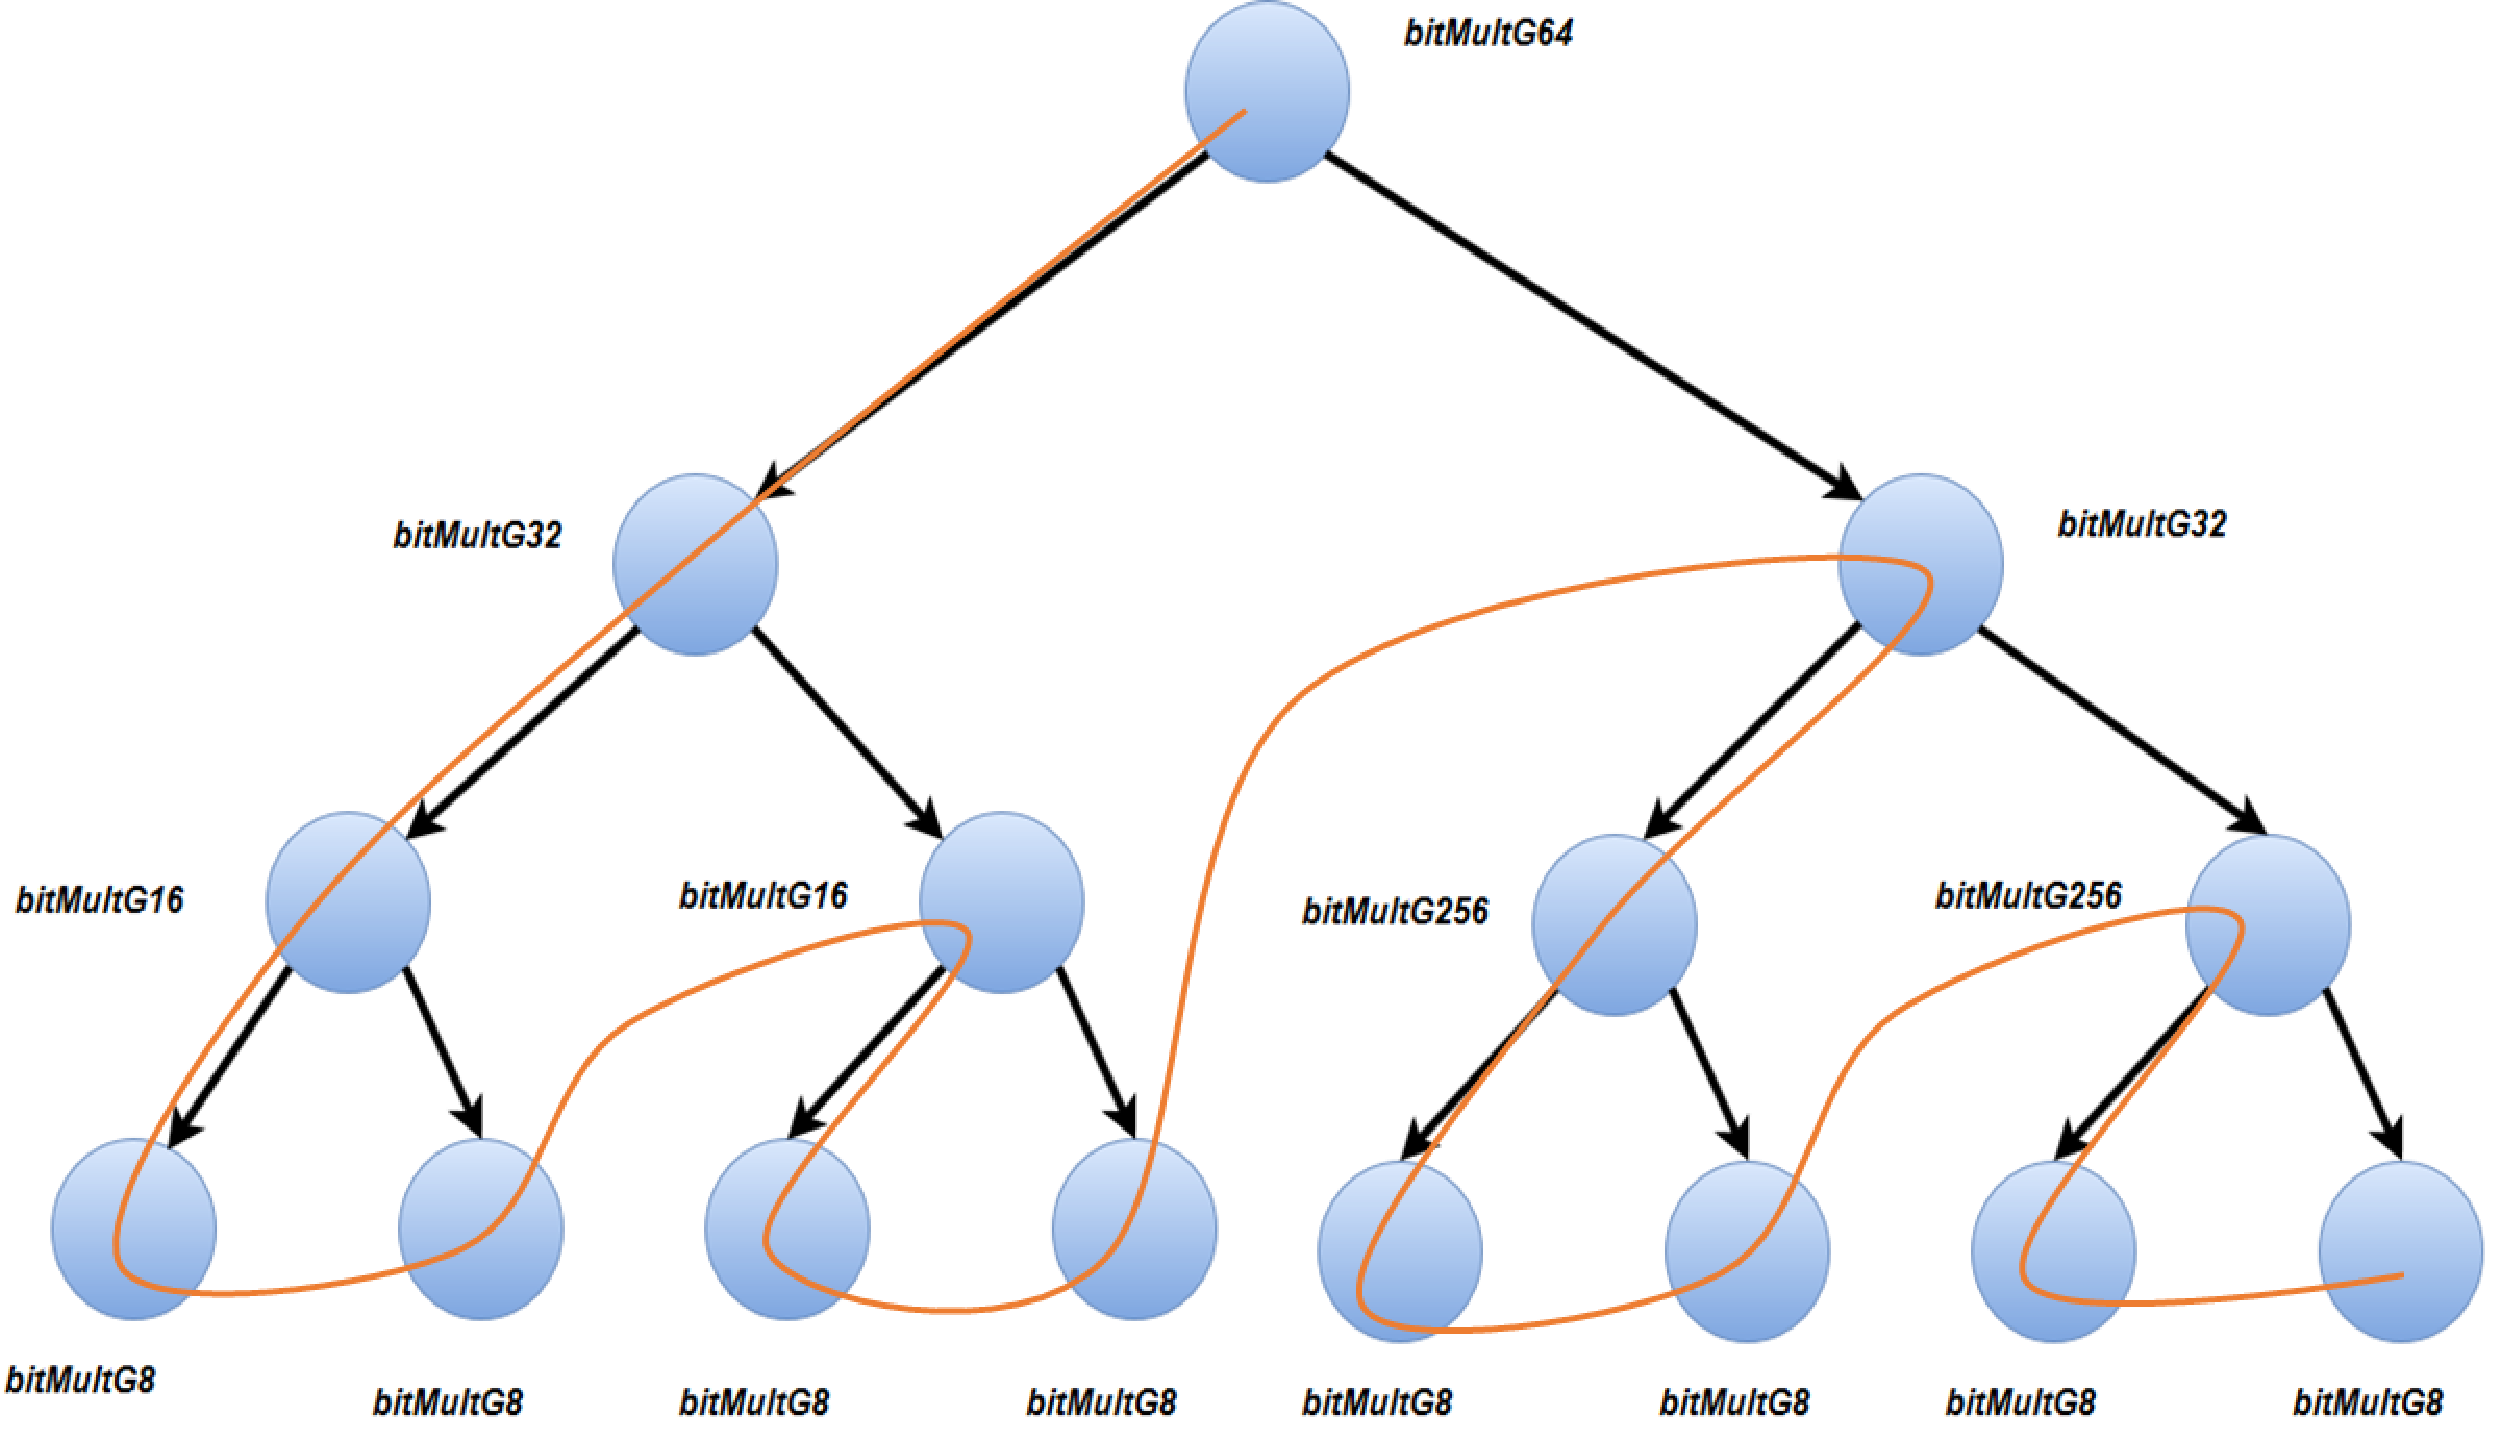
\includegraphics[width=0.7\textwidth]{./figures/unrolledEncoder.pdf}
	\caption{Pruned unrolled encoder tree}
	\label{fig:unrolledEncoder}
\end{figure}

Sample code snippet of node operation with SIMD instructions is shown in listing ~\ref{code:NodeOperation}.

\begin{code}
	\captionof{listing}{Node operation using SIMD instructions}
	\label{code:NodeOperation}
\begin{minted}[frame=single]{c}
inline void bitMultG512(uint8_t *s, uint8_t *dEncoded) 
{
	//Here s is 64 bytes, Divided to 32 bytes each.
	uint8_t *s1 = (uint8_t *) s;
	uint8_t *s2 = (uint8_t *) (s + 32);
	__m256i result;
	__m256i temp1 = _mm256_loadu_si256((__m256i*)operand1);
	__m256i temp2 = _mm256_loadu_si256((__m256i*)operand2);
	result = _mm256_xor_si256(temp1,temp2);
	_mm256_storeu_si256((__m256i*)destn, result);
	bitMultG256((uint8_t *) s1, dEncoded);
	bitMultG256((uint8_t *) s2, dEncoded);
}
\end{minted}
\end{code}

\begin{table}[!h]
	\begin{center}
		\caption{Latency comparison: polar encoding for 1024 bits}
		\label{tab:polarEncoder}
		\begin{tabular}{c|c|c} % <-- Alignments: 1st column left, 2nd middle and 3rd right, with vertical lines in between
			\textbf{ } & Naive & Optimized \\
			\hline
			Latency ($\mu$s) & $34$ & $0.244$\\
		\end{tabular}
	\end{center}
\end{table}


\section{Sub-block interleaver}
Subblock interleaver divides the block of $N$ bits into $32$ subblocks, each containing $\frac{N}{32}$ bits. These subblocks are interleaved as shown in Figure \ref{fig:subblockInterleaver}. Functionally, subblock interleaving is implemented with algorithm presented in \cite{3gpp.38.212}. Computation complexity of interleaving indexes is huge due to the use of multiplication, division and modulus operations. For a subblock interleaver block, minor optimizations such as avoiding expensive operations such as multiplication/division/modulus and replacing them with right or left shift operations are performed.

\section{Rate matching}
Rate matching block calculates $E$ bits out of $N$ bits. Value of $E$ relative to $N$ determines the mode of rate matching. There can be three modes namely repetition, shortening and puncturing. For the scenarios where $E \geq N$ repetition is applied otherwise either puncturing or shortening needs to be done. Through empirical measurements, it is found that for high rates shortening performs better and puncturing for low rates. Rate matching is performed by a circular buffer as given in \cite{DesignOfPolarCodes5G}. Major optimization in rate matching block is avoiding copy operations instead change the pointers for cases shortening/puncturing and repetition. Minor optimizations include using compiler primitives as hints to reduce the branchings and copying data blockwise instead of element-wise for repetition mode of rate matching. Blockwise copying is efficient since it can employ SIMD instructions and also it avoids usage of modulus operation in repetition mode.

\section{Channel interleaver}
The 5G standard specifies channel interleaver for higher order modulations for better error correction performance \cite{3gpp.TSG-RAN_WG1}. In the downlink, PBCH/PDCCH use only QPSK, hence channel interleaving is disabled using a parameter $I\_BIL$. Setting it to zero disables the channel interleaver. For uplink channels such as PUCCH/PUSCH, higher modulations can be used. In those scenarios, channel interleaving is enabled. This work focuses mainly on PDCCH/PBCH channels so interleaving block contribution to latency is zero since it is disabled. There are no optimizations performed for this block in the FEC chain.

\section{Miscellaneous optimizations}
In addition to the above described major improvements, many micro-optimizations are performed. Few examples are \newline
$\bullet $ Avoiding multiplication/division/modulus operations and achieving the same using bitwise operators.\newline
$\bullet $ Implemented approximate versions $\log_2{(x)}$ and $\exp{(x)}$ functions to reduce the number of floating point multiplications.\newline
$\bullet $ Avoided jump functions to reduce flushing of the instruction pipeline.\newline
$\bullet $ Using the compiler optimization primitives to reduce branches in the program.\newline

\section{Results Comparison}

\subsubsection{PBCH FEC chain}
Parameters of the FEC chain are \newline
$n_{max} = 9, I_{IL} = 1, n_{pc} = 0, n_{pc}^{wm} = 0, I_{BIL} = 0, L = 24, E = 864, K = 56$
\begin{table}[!h]
	\begin{center}
		\caption{Latency comparison: PBCH FEC chain}
		\label{tab:pbchFecChain}
		\begin{tabular}{c|c|c} % <-- Alignments: 1st column left, 2nd middle and 3rd right, with vertical lines in between
			\textbf{ } & Naive & Optimized \\
			\hline
			Latency ($\mu$s) & $53$ & $7$\\
		\end{tabular}
	\end{center}
\end{table}

%\NOTE{PBCH with google benchmark naive = 30us, Optimized = 2.3us, Google benchmark gives reliable reproducible numbers average}
\subsubsection{PDCCH FEC chain} 
In case of PDCCH reliability indices need to be identified at runtime due to varying $A$, $N$, and $E$. PDCCH latency gives an overall picture of employed optimizations. Parameters of the FEC chain are \newline
$n_{max} = 9, I_{IL} = 1, n_{pc} = 0, n_{pc}^{wm} = 0, I_{BIL} = 0, L = 24, E = 423, K = 106$
\begin{table}[!h]
	\begin{center}
		\caption{Latency comparison: PDCCH FEC chain}
		\label{tab:pdcchFecChain}
		\begin{tabular}{c|c|c} % <-- Alignments: 1st column left, 2nd middle and 3rd right, with vertical lines in between
			\textbf{ } & Naive & Optimized \\
			\hline
			Latency ($\mu$s) & $162$ & $19$\\
		\end{tabular}
	\end{center}
\end{table}

%\NOTE{PDCCH with google benchmark naive = 104us, Optimized = 7.2us, Google benchmark gives reliable reproducible numbers average} \newline

To obtain overall picture of improvement from all the above optimizations it is worthwhile to look at worst case latencies of the FEC chain which is with maximum block size ($N = 1024$), with puncturing (requires more time to identify reliability indices as well as for rate matching) and with both input bit-interleaving and channel-interleaving. Following table gives a comparison between naive and optimized versions.

Worst case latency FEC chain parameters, \newline
$I_{IL} = 1, n_{max} = 10, n_{pc} = 0 ,n_{pc}^{wm} = 0, I_{BIL} = 1, E = 846, K = 106$.
\begin{table}[!h]
	\begin{center}
		\caption{Worst case latency comparison: Polar FEC chain}
		\label{tab:worstFecChain}
		\begin{tabular}{c|c|c} % <-- Alignments: 1st column left, 2nd middle and 3rd right, with vertical lines in between
			\textbf{ } & Naive & Optimized \\
			\hline
			Latency ($\mu$s) & $451$ & $40$\\
		\end{tabular}
	\end{center}
\end{table}

\section{Summary}
In this section, we implemented the polar encoding FEC chain. Different components of the FEC chain are analyzed to understand the complexity and latency contributions. Through extensive analysis and code profiling, three major latency contributors are identified, namely CRC calculation, polar code construction, and polar encoding. All these components are optimized using algorithmic and platform-specific optimizations. The latency of CRC calculation is reduced by using lookup and exploiting the data parallelism. The biggest contributor to latency in the FEC chain is the polar code construction due to the presence of expensive search, remove and copy operations. The polar code construction algorithm is reformulated to reduce latency by avoiding above mentioned expensive operations. Polar encoding is another latency contributor. The encoder is optimized using a number of techniques. Significant optimizations include pruning encoder tree, implementing encoding with SIMD instructions, unrolling the recursive function and by avoiding superfluous copy operations. All the above-mentioned optimizations to FEC chain reduced the latency by 10x compared to naive implementation.